\documentclass[12pt,a4paper]{scrartcl}
\usepackage[utf8]{inputenc}
\usepackage[english,russian]{babel}
\usepackage{indentfirst}
\usepackage{misccorr}
\usepackage{graphicx}
\usepackage{amsmath}
\usepackage{multirow}
\usepackage{pgfplots}
\usepackage{parskip}
\usepackage[top=1cm, bottom=1cm, left=1cm, right=1cm]{geometry}
\pgfplotsset{compat=1.9}

\begin{document}
	\graphicspath{{py/}}
	
	\newcommand{\ms}{\mathstrut}
	\newcommand{\msp}{\hspace{0.5cm}}
	\newcommand{\al}{\alpha}
	\newcommand{\dg}{^\circ}
	\newcommand{\dif}{\mathrm{d}}
	\newcommand{\qd}[2]{^{\frac{#1}{#2}}}
	\newcommand{\qdm}[2]{^{-\frac{#1}{#2}}}
	\newcommand{\lm}[2]{\underset{#1 \rightarrow #2}{\lim}}
	\newcommand{\sfrac}[2]{\dfrac{\strut #1}{\strut #2}}
	\newcommand{\equal}[1]{\overset{(#1)}{=}}
	\newcommand{\linevdots}{\ \raisebox{-.08\height}{\vdots}\ }
	\newcommand{\linecvdots}{\ \raisebox{-.08\height}{\vdots}\hspace{-0.13cm}\raisebox{.15\height}{\cancel{\phantom{a}}\hspace{0.06cm}}}
	\newcommand{\combox}[1]{\ms \msp \msp \begin{minipage}{0.95\linewidth}
			#1
	\end{minipage}}
	
	\newtheorem{pr}{Задача}
	\newtheorem{ex}{Пример}
	\newtheorem{dfn}{Def}
	\newtheorem{theorem}{Th}
	
	\newenvironment{slv}{\ms \msp \textit{Решение:}}{}
	\newenvironment{proof}{\ms \msp \textit{Доказательство: }}{\hfill $\square$}
	
	\begin{titlepage}
		
		\vspace*{\fill}
		
		\begin{center}
			
\includegraphics[scale=0.8]{MIPT.png}
			\\[0.7cm]\Huge Московский Физико-Технический Институт\\(национальный исследовательский университет)
			\\[2cm]\LARGE Отчет по эксперименту
			\\[0.5cm]\noindent\rule{\textwidth}{1pt}
			\\\Huge\textbf{Вынужденные колебания в электрическом контуре}
			\\[-0.5cm]\noindent\rule{\textwidth}{1pt}
		\end{center}
		
		\begin{flushleft}
			\textit{Работа №3.2.5; дата: 02.09.22}\hfill\textit{Семестр: 3}
		\end{flushleft}
		
		\vspace*{\fill}
		
		\begin{flushleft}
			Выполнил: \hspace{\fill} Группа:
			\\Кошелев Александр \hspace{\fill} Б05-105
		\end{flushleft}
	\end{titlepage}
	
	%Страница 2
	
	\begin{flushleft}
		\footnotesize{Вынужденные колебания в электрическом контуре} \hspace{\fill} \footnotesize{2}
		\\[-0.3cm]\noindent\rule{\textwidth}{0.3pt}
	\end{flushleft}
	
	\section{Аннотация}
	
	\textbf{Цель работы: }
	
	Исследование вынужденных колебаний и процессов их установления в колебательном контуре.
	
	\textbf{Схема установки:}
	\begin{center}
		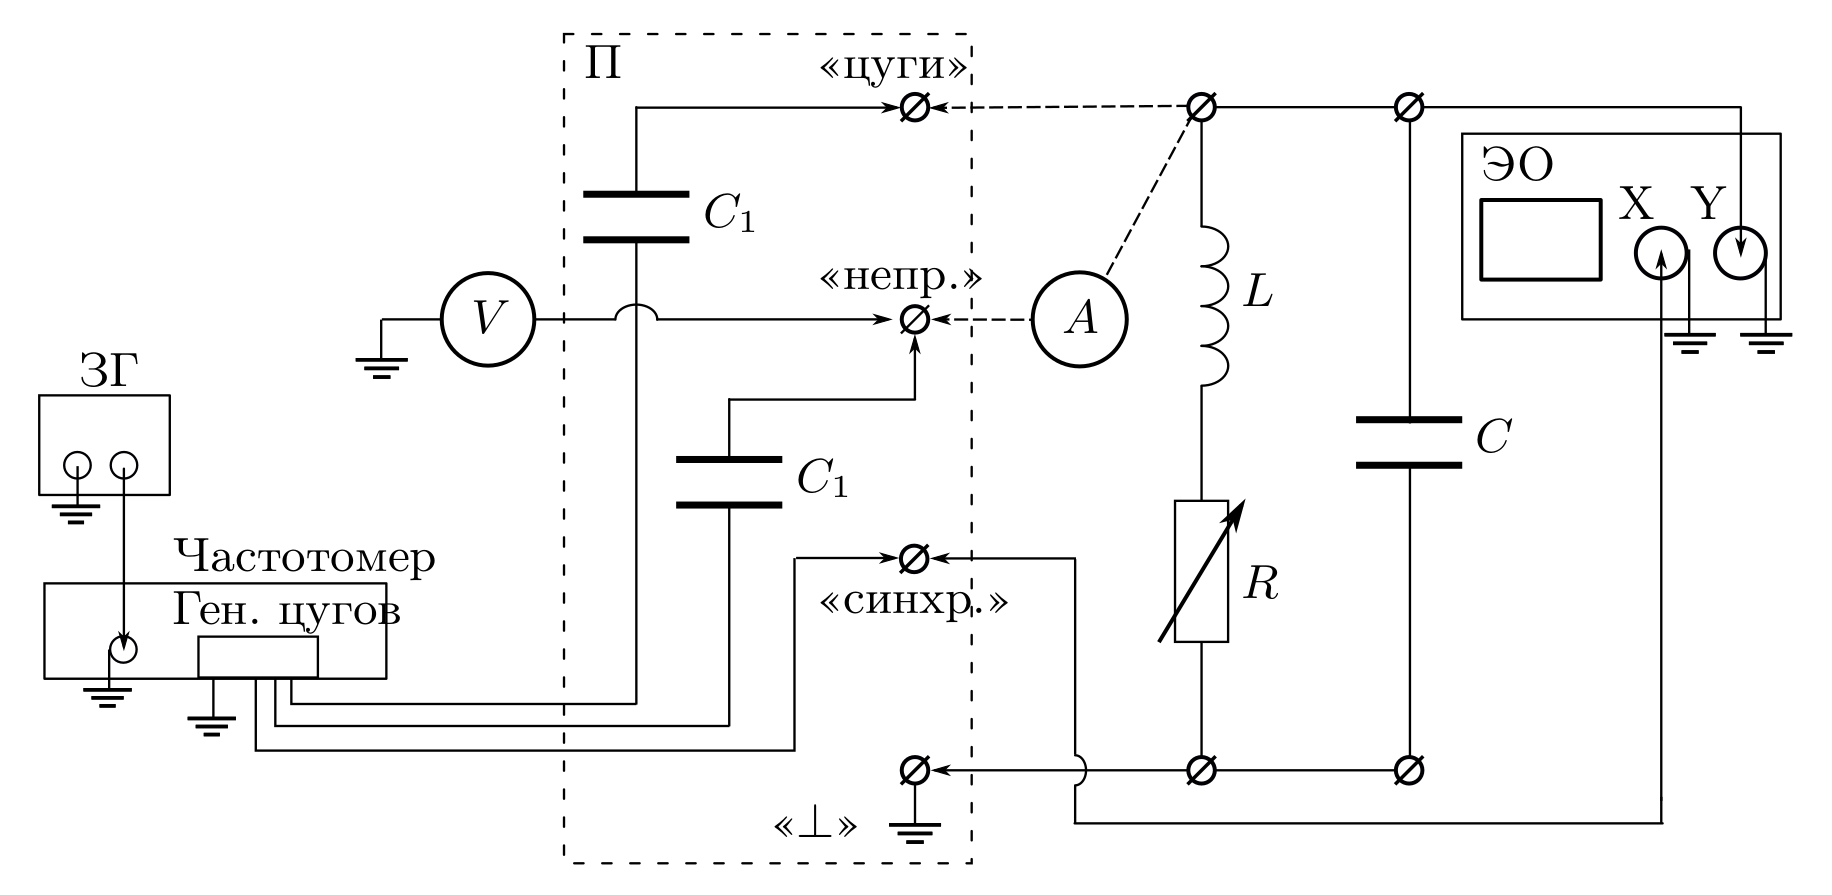
\includegraphics[scale=0.2]{PIC_1}
		\\\textbf{Рис. 1:} Схема установки
	\end{center}	
		
	\textbf{В работе используются:}
	
	Генератор звуковых частот, вольтметр, частотомер, конденсатор, катушка индуктивности, магазин сопротивлений, осциллограф, универсальный измеритель импеданса ($LCR$-метр).
	
	\section{Теоретические сведения}
	Для экспериментального исследования резонансной кривой тока в последовательном колебательном контуре можно снять зависимость амплитуды напряжения на резситоре $R$ от частоты генератора (при постоянной амплитуде выходного напряжения генератора). Но импеданс этого контура включает в себя выходной импеданс генератора. Мы должны быть уверены, что выходной импеданс генератора много меньше импеданса контура и не влияет на процессы, происходящие в этом контуре.
	
	Для устранения этого влияния можно использовать схему, представленную на Рис. 2: синусоидальный синал с генератора подаётся на параллельный колебательный контур через небольшую разделительную ёмкость $C_1$. Напряжение с ёмкости контура $C$ поступает на вертикальный вход ЭО.
	
	\begin{center}
		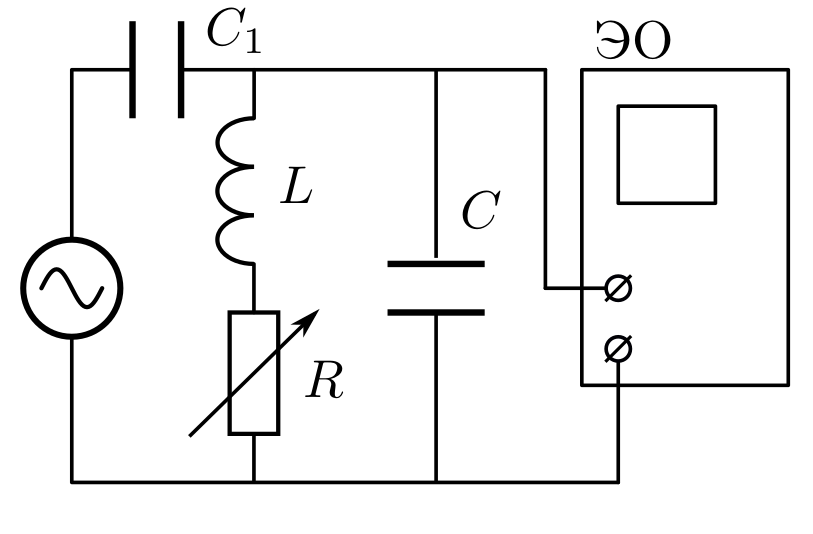
\includegraphics[scale=0.2]{PIC_2}
		\\\textbf{Рис. 2:} Схема установки
	\end{center}
	
	\newpage 
	
	%Страница 3
	
	\begin{flushleft}
		\footnotesize{Вынужденные колебания в электрическом контуре} \hspace{\fill} \footnotesize{3}
		\\[-0.3cm]\noindent\rule{\textwidth}{0.3pt}
	\end{flushleft}
	
	Зависимость амплитуды этого напряжения от частоты генератора будет практически совпадать с резонансной кривой для последовательного контура, если импедансы возбуждающей и измеряющей цепей (сопротивления переменному току) намного превосходят импеданс самого контура вблизи резонанса $Z_\text{рез} \approx L / (RC) = Q / (\Omega C)$. Разделительная ёмкость $C_1$ выбирается настолько малой, что в рабочем диапазоне частот её импеданс $Z_{C_1} = 1/(\Omega C_1)$ много меньше импеданса контура, поэтому в цепи генератора течёт ток практически с постоянной амплитудой, а колебательный контур выполняет роль нагрузочного сопротивления, которое, в свою очередь, зависит от частоты. Поскольку в резонансе сопротивление $Z_\text{рез}$ параллельного контура максимально, то и напряжение на ёмкости $C$ (неизменный ток, умноженный на максимальное сопротивление) тоже максимально. Входное сопротивление осциллографа (измеряющей цепи) достаточно велико: $R_\text{ЭО} \approx 1 \text{МОм}$.
	
	Таким образом, при выполнении условий

	$$Z_{C_1} = \frac{1}{\Omega C_1} \gg |Z| = \frac{Q}{\Omega C}, \quad R_\text{ЭО} \gg \frac{Q}{\Omega C}$$
	
	и при условии, что действительная часть импеданса катушки много меньше её мнимой части, резонансная кривая в нашем контуре бует выглядеть так же, как в последовательном: максимум амплитуды при резонансе. Ширина резонансной кривой определяет важную характеристику контура --- добротность.
	
	Добротность контура может быть определена и другими способами, например, по скорости нарастания амплитуды вынужденных колебаний при резонансе или по скорости затухания свободных колебаний. Нарастание и затухание колебаний можно наблюдать на экране осциллографа, если на контур подаются цуги --- отрезки синусоиды, разделённые интервалами, в течение которых сигнал отсутствует. Чем выше добротность, тем медленне нарастают и медленнее затухают колебания в контуре. Количественные оценки можно сделать, сли определить логарифмический декремент затухания по скорости нарастания или затухания колебаний. В условиях резонанса огибающая затухающих колебаний это перевёрнутая огибающая нарастающего участка, поэтому при расчёте логарифмического декремента по затуханию нет необходимости использовать амплитуду установившихся колебаний $U_0$, которая в контуре с высокой добротностью иногда не успевает установиться за время продолжительности цуга.
	
	
	\section{Проведение эксперимента}
	
	\paragraph{Определение добротности методом резонансных кривых} \hfill
	
	Вначале теоретически рассчитаем резонансную частоту контура по соответствующей формуле для $LC$-контура:
	
	$$\nu_{\text{теор}} = \sfrac{1}{2\pi LC} \approx 1592\, \mathrm{Hz}$$
	
	Замеры на контуре будем производить при двух значениях нагрузочного сопротивления $R_1 = 0\, \mathrm{Ohm}$ и $R_2 = 100\, \mathrm{Ohm}$.
	
	\begin{center}
		\begin{tabular}{|c|c|c|c|c|c|c|c|c|c|}
			\hline $\nu \pm 0.001, kHz$ & 1.360 & 1.408 & 1.443 & 1.468 & 1.493 & 1.516 & 1.538 & 1.551 & 1.575
			\\\hline $U, V$ & 1.42 & 1.78 & 2.21 & 2.63 & 2.98 & 3.40 & 3.81 & 4.00 & 4.15
			\\\hline $\nu \pm 0.001, kHz$ & 1.616 & 1.653 & 1.682 & 1.700 & 1.717 & 1.742 & 1.766 & 1.794 & 1.841
			\\\hline $U, V$ & 3.92 & 3.39 & 3.00 & 2.82 & 2.57 & 2.40 & 2.19 & 1.99 & 1.82
			\\\hline
		\end{tabular}
		\\\textbf{Табл. 1:} Измерения при $R_1 = 0\, \mathrm{Ohm}$
	\end{center}
	
	\newpage
	
	%Страница 4
	
	\begin{flushleft}
		\footnotesize{Вынужденные колебания в электрическом контуре} \hspace{\fill} \footnotesize{4}
		\\[-0.3cm]\noindent\rule{\textwidth}{0.3pt}
	\end{flushleft}

	\begin{center}
		\begin{tabular}{|c|c|c|c|c|c|c|c|c|c|}
			\hline $\nu \pm 0.001, \mathrm{kHz}$ & 1.522 & 1.530 & 1.537 & 1.540 & 1.548 & 1.555 & 1.561 & 1.567 & 1.575
			\\\hline $U, \mathrm{V}$ & 7.2 & 8.4 & 9.4 & 10.2 & 12.1 & 13.9 & 16.0 & 18.1 & 18.6
			\\\hline $\nu \pm 0.001, \mathrm{kHz}$ & 1.581 & 1.587 & 1.593 & 1.600 & 1.608 & 1.613 & 1.618 & 1.627 & 1.634
			\\\hline $U, \mathrm{V}$ & 17.9 & 16.1 & 14.0 & 12.2 & 9.8 & 9.6 & 8.8 & 7.6 & 6.8
			\\\hline
		\end{tabular}
		\\\textbf{Табл. 2:} Измерения при $R_2 = 100\, \mathrm{Ohm}$
	\end{center}
	
	Приведем и графики резонансных кривых:
	
	\begin{center}
		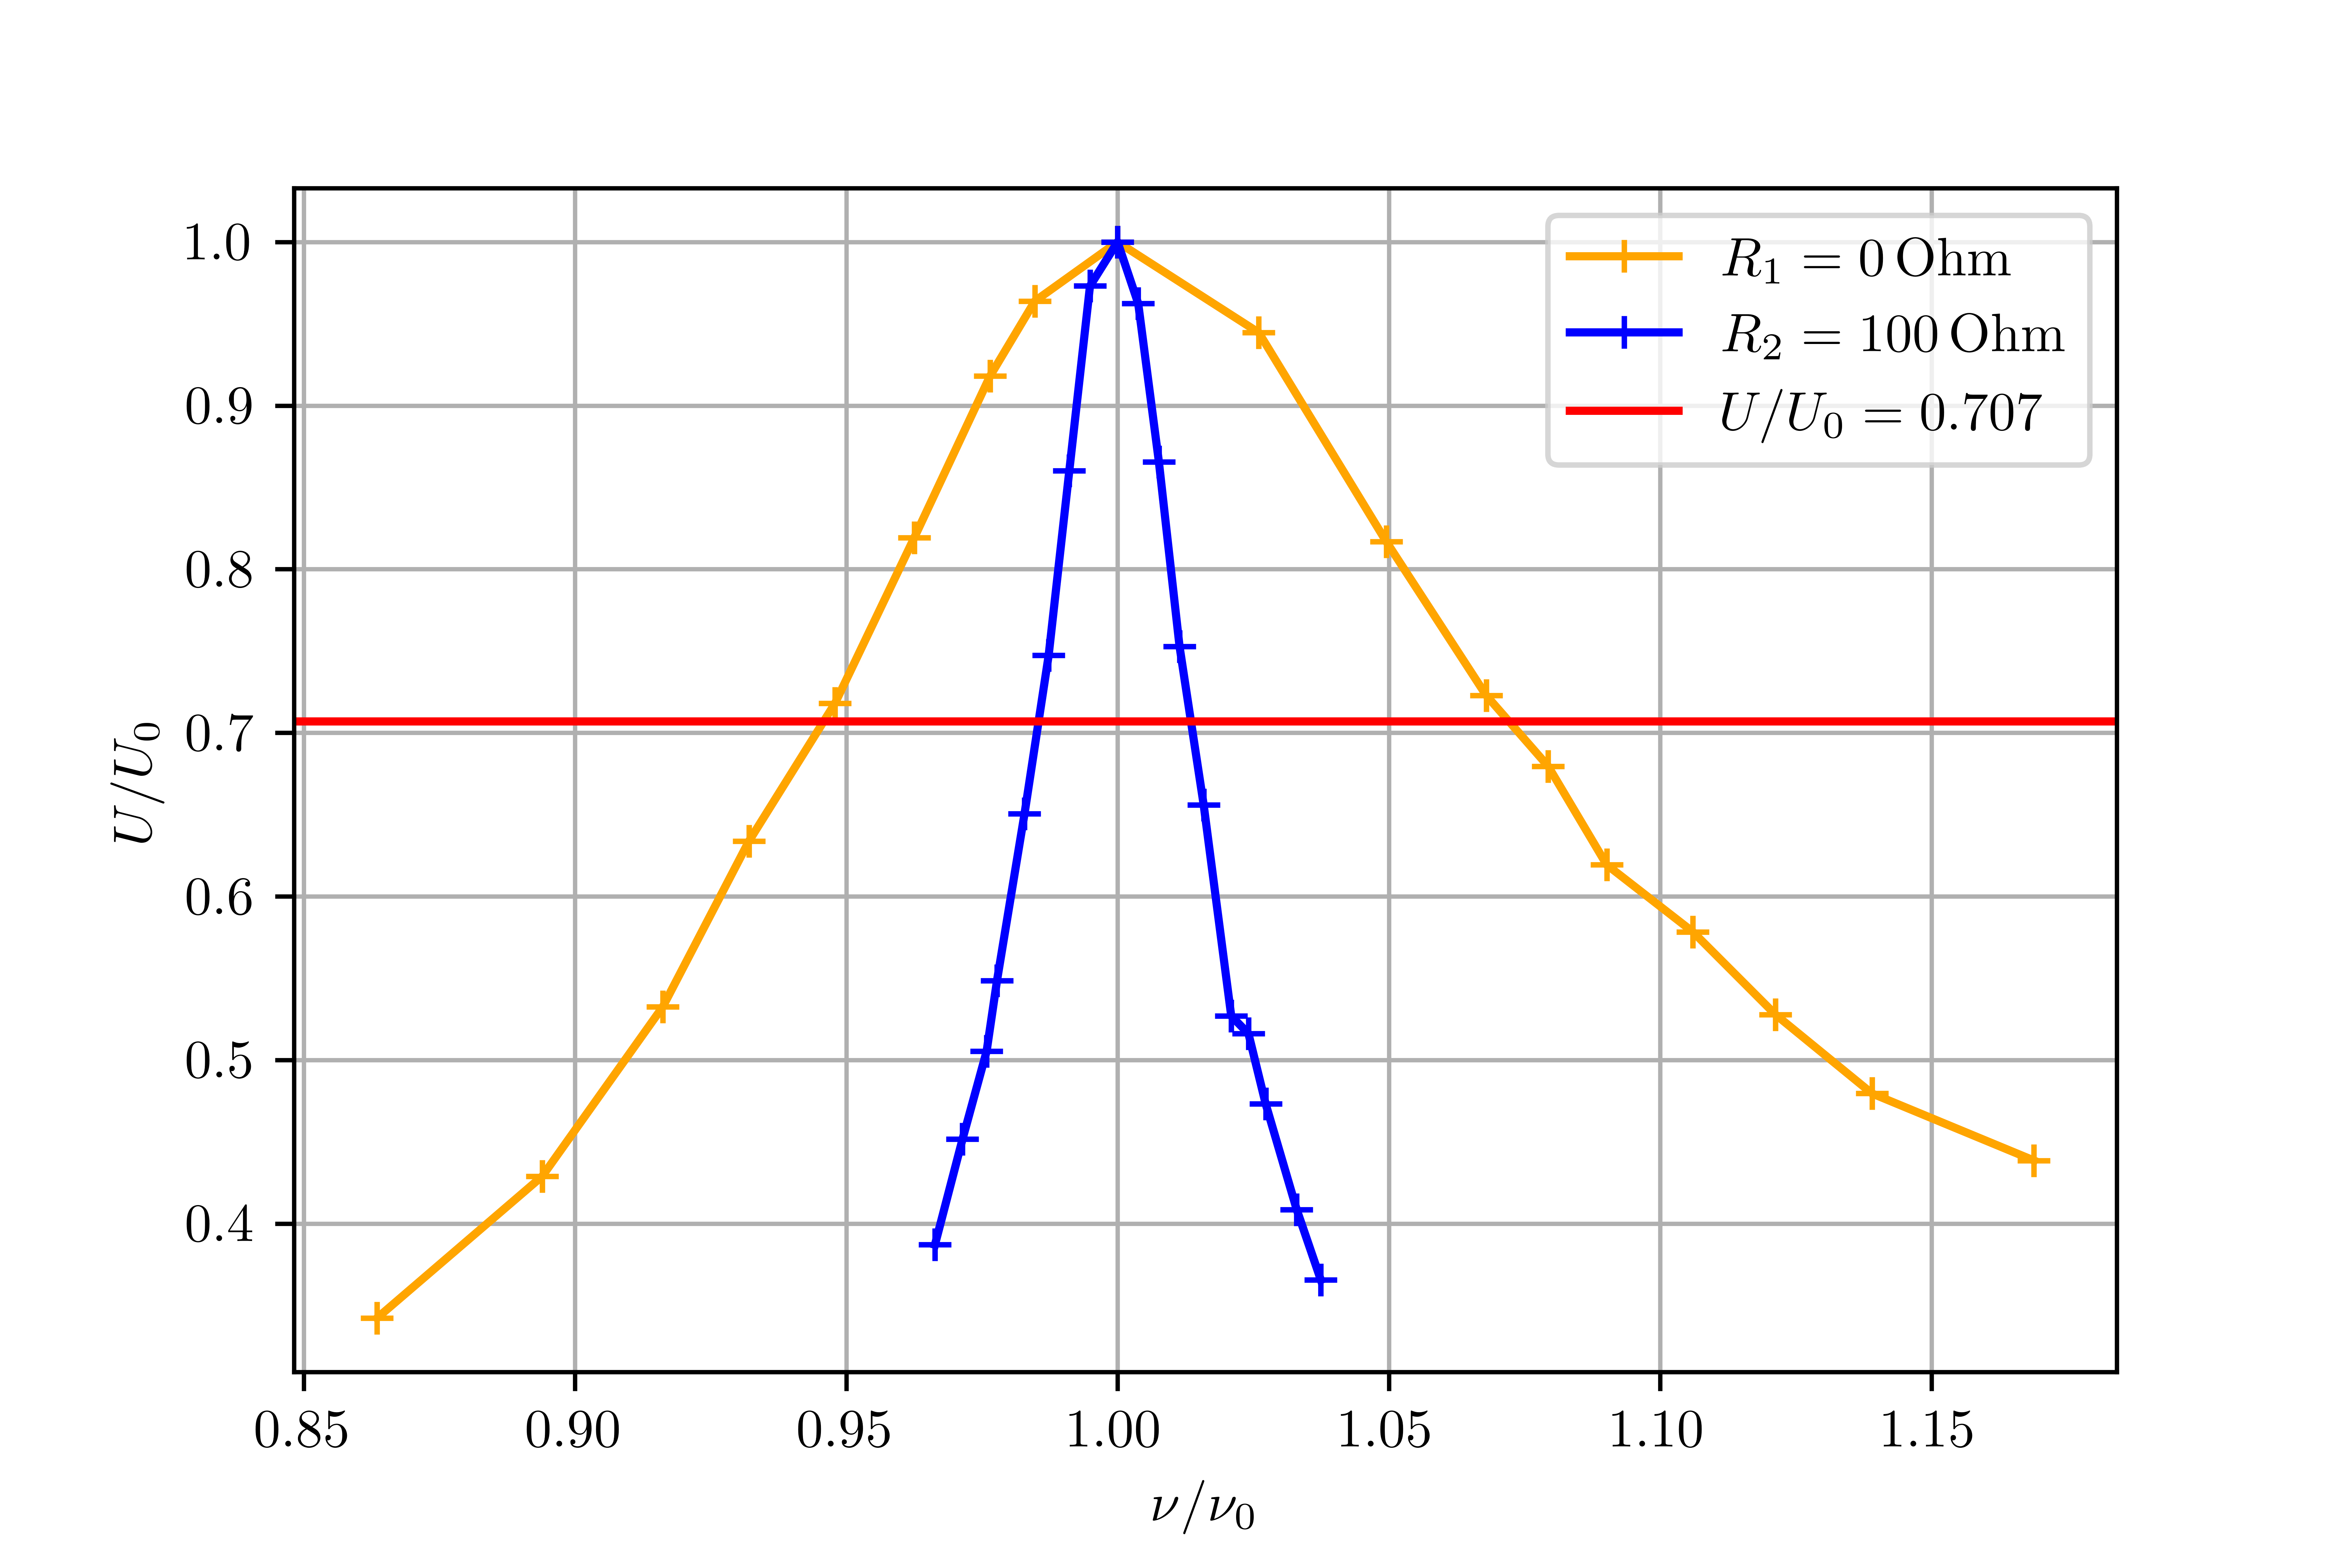
\includegraphics[scale=1]{PIC_3.png}
		\\\textbf{Рис. 3:} Резонансные кривые
	\end{center}

	Теперь рассчитаем добротность из данных графика по формуле:
	
	$$Q_{0} = \sfrac{\omega_0}{\delta{\omega}} = \sfrac{1}{\delta(\nu / \nu_0)} \approx 28 \pm 2\ \ \ \ \ Q_{100} \approx 7.8 \pm 0.6$$
	
	\paragraph{Определение добротности по нарастанию и затуханию} \hfill
	
	Перейдем к подаче цуг на контур, и запишем данные затухания и нарастания:
	
	\begin{center}
		\begin{tabular}{|c|c|c|c|c|c|c|c|c|}  \hline
			{} & \multicolumn{4}{|c|}{Нарастание} & \multicolumn{4}{|c|}{Затухание} \\\hline
			$U_k,\ \text{units}$ & 12 & 12 & 14 & 20 & 30 & 29 & 29 & 28 \\\hline
			$U_{k+n}, \text{units}$ & 14 & 20 & 26 & 30 & 27 & 24 & 26 & 23 \\\hline
			$n$ & 1 & 4 & 7 & 8 & 3 & 4 & 3 & 4 \\\hline
			$Q$ & 36.1 & 30.9 & 27.9 & 25.6 & 25.2 & 23.3 & 26.4 & 25.9 \\\hline
			$\sigma Q$ & 2.8 & 2.4 & 2.0 & 2.1 & 1.7 & 1.6 & 1.7 & 1.7 \\\hline
		\end{tabular}
		\\\textbf{Табл. 3:} Нарастание и затухание при $R_1 = 0\, \mathrm{Ohm}$
	\end{center}
	
	\newpage
	
	%Страница 5
	
	\begin{flushleft}
		\footnotesize{Вынужденные колебания в электрическом контуре} \hspace{\fill} \footnotesize{5}
		\\[-0.3cm]\noindent\rule{\textwidth}{0.3pt}
	\end{flushleft}
	
	\begin{center}
		\begin{tabular}{|c|c|c|c|c|c|c|c|c|}  \hline
			{} & \multicolumn{4}{|c|}{Нарастание} & \multicolumn{4}{|c|}{Затухание} \\\hline
			$U_k,\ \text{units}$ & 10 & 19 & 28 & 33 & 32 & 27 & 33 & 37 \\\hline
			$U_{k+n}, \text{units}$ & 18 & 32 & 36 & 38 & 15 & 9 & 9 & 5 \\\hline
			$n$ & 2 & 2 & 2 & 2 & 2 & 2 & 3 & 5 \\\hline
			$Q$ & 7.6 & 7.6 & 7.4 & 7.7 & 6.3 & 8.7 & 7.3 & 7.8 \\\hline
			$\sigma Q$ & 1.1 & 1.0 & 0.9 & 0.9 & 0.7 & 1.1 & 1.0 & 1.1 \\\hline
		\end{tabular}
		\\\textbf{Табл. 4:} Нарастание и затухание при $R_2 = 100\, \mathrm{Ohm}$
	\end{center}

	Теперь усредним полученные данные, и запишем их в виде таблицы:
	
	\begin{center}
		\begin{tabular}{|c|c|c|} \hline
			$R,\, \mathrm{Ohm}$ & $Q_\text{воз}$ & $Q_\text{зат}$ \\\hline
			$0$ & $30.1 \pm 2.2$ & $25.2 \pm 1.8$ \\\hline
			$100$ & $7.5 \pm 0.9$ & $7.6 \pm 0.9$ \\\hline 
		\end{tabular}
		\\\textbf{Табл. 5:} Итоговая добротность по возрастанию/затуханию
	\end{center}
	
	\section{Выводы}
	
	Для демонстрации выводов составим таблицу по рекоммендации из задавальника:
	
	\begin{center}
		\begin{tabular}{|c|c|c|c|c|c|} \hline
			$R,\, \mathrm{Ohm}$ & $R_\text{акт},\, \mathrm{Ohm}$ & $Q_\text{граф}$ & $Q_\text{воз}$ & $Q_\text{зат}$ & $Q_\text{теор}$ \\\hline
			$0$ & $25.075$ & $28 \pm 2$ & $30.1 \pm 2.2$ & $25.2 \pm 1.8$ & $25.7 \pm 1$ \\\hline
			$100$ & $25.075$ & $7.8 \pm 0.6$ & $7.5 \pm 0.9$ & $7.6 \pm 0.9$ & $7.7 \pm 0.5$ \\\hline 
		\end{tabular}
		\\\textbf{Табл. 6:} Результаты
	\end{center}

	Полученные экспериментально значение добротности с учетом погрешности совпадает с теоретическим. Данные графического метода могли бы быть уточнены при более точной аппроксимации частотных кривых соответствующими функциями.
	
\end{document}